\chapter{Security}
\minitoc

\section{Lab Description}
\textit{The main objective of this week's assignment is to understand and analyze security models and protocols and furthermore implement a simple security protocol for task manager. As part of the assignment, you will study and develop a simple role based access control mechanism for tasks based on an authentication using ITU credentials. Moreover, you will also use one of the crypto algorithms to ensure security among all/some parts of communication.}

\section{Solution}

The handed-out project implements a simple security protocol. There's no way for the server to authenticate the messages from the client and vice versa. The challenge in the assignment is to implement an improved protocol that, among other things, allows a client and a server to exchange a shared secret key which then facilitates authenticated communication between them. Thus providing slightly better security.  \\

The project uses shared private keys between participants i.e., the keys are already distributed between the participants. Token server and client share a private key and so does token server and server and also server and client. The challenge is how to implement a way for the client and server to share a secret key (session key) with which they can communicate in a secure way. \\

First, the client sends a request to the authentication server (token server). The token server sends back a encrypted response inside which is a ticket encrypted in the token-server key plus a session key for the communication between the client and the server. \\

\begin{lstlisting}
// from client to token server
{ credentials }K_tc
// from token service to client
{ {role, timestamp, identity, session key}K_ts, session key} 
\end{lstlisting}

The client is able to decrypt the response with the already distributed [token server-client] shared private key. The ticket is encrypted in the [token server-server] shared private key and contains the [client-server] shared key (the session key) plus the clients identity, plus a timestamp and the clients role(note the server later uses the role to authenticate the client against an access rights table restricting access to it's resources). \\ 

If this message is intercepted the encryption with the clients private key poses a challenge to the enemy but crucially, if the enemy manages to send the message to the server posing as the client, it is of no matter as the server then compares the identity in the ticket against the sender, if they do not match the server denies access to its resources.\\

Second, the client sends a 'authenticate' request to the server along with the ticket encrypted in the servers private key. The server decrypts the message and authenticates the client against the identity in the ticket. The session key has now been distributed between the server and client and will be used for communication between them. The server sends a reply consisting of a message and a nonce encrypted with the server-client shared key (the session key). Further communication between client and server is to be authenticated  against that nonce.
\begin{lstlisting}
// from client to server
authenticate, {role, timestamp, identity, session key}K_ts 
// from server to client
if(authenticated)
	yes, { nonce }K_sc
else
	no, {message}K_sc
\end{lstlisting}

When the server later receives a message from the client it contains that nonce transformed by some agreed upon function (in this case simply the nonce - 1). By applying the transformation to the nonce the client effectively authenticates it's identity to the server. \\

Using a nonce like this adds another layer of security. If an enemy intercepts the message it will need to first deal with the session key after which it will still need to know which transformation of the nonce is the correct one in order to continue communicating with the server. \\

Only now do the client send a resource request to the server. the request message consists of a command plus the transformed nonce encrypted in the client-server shared key plus the data on which to act, also encrypted in the shared key. \\

The server validates the transformed nonce and the clients role against the access rights table, and finally it checks the message timestamp. It replies by sending a message and yet a transformed nonce (the nonce could possibly be a new transformation of the same nonce?) on which further client-server communication is based.

%\pagebreak

\begin{lstlisting}
// from client to server
execute, {transformed nonce}K_sc, {data}K_sc
// from server to client
if(succesful execute)
	yes, {another nonce}K_sc
else
	no, {message}K_sc
\end{lstlisting}

In this rather convoluted way the server and client now has obtained a shared private key on which to communicate (more) securely. The example still relies on a trusted third party, the principles involved still need to initially share secret keys. So in the end there remains the need for some trusted source, some authentication service. \\
 
\begin{comment}
There's also still the possibility of a man-in-the-middle attack in where the message form the token server is send to the enemy, but ... 
\end{comment}

%\pagebreak

\section{Example run}

\begin{center}
\centering
\caption{example run}
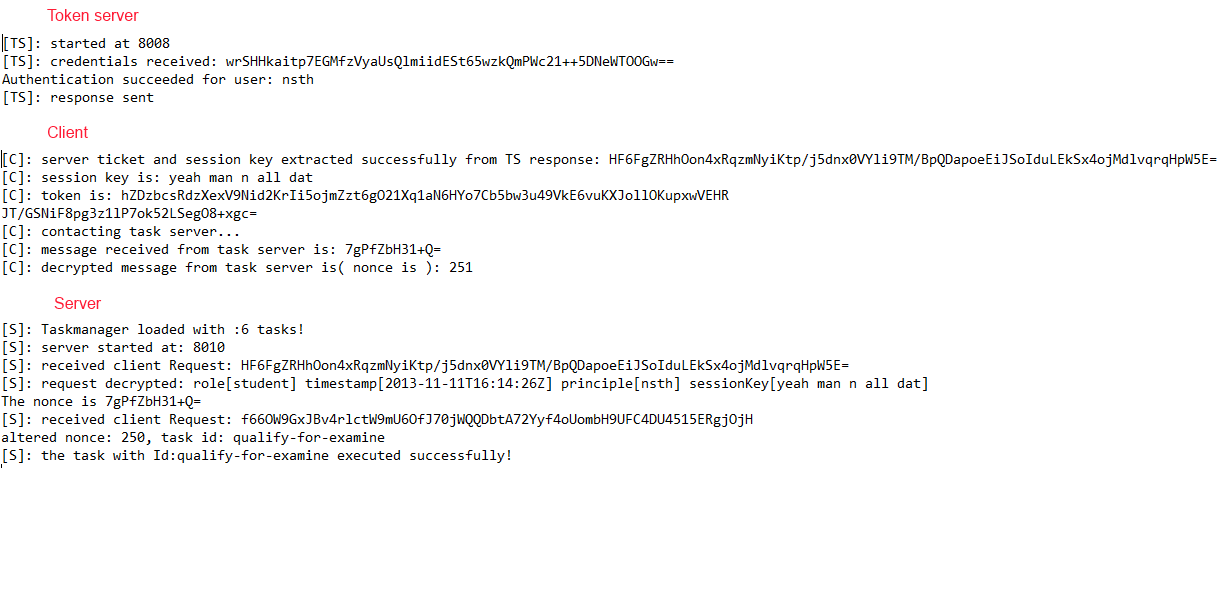
\includegraphics[scale=0.5]{images/security_run.png}
\end{center}
\vspace{10pt}

\section{Theory}


The solution to security issues in distributed systems is to encrypt messages. All encryption algorithms are based on using a secret (called a key). Encryption algorithms use the key to obscure the content of messages (encrypt the message), and to decrypt the message using the same key. There are two types of keys and thus two types of encryption algorithms: \\

\begin{itemize}
\item[  \textbf{shared secret keys:}] In which both the sender and the receiver knows the secret, note \textit{this is a typical army or corporate solution in that these organizations are able to distribute the secret key, secretely.}

\item[\textbf{public/private key pairs:}] In which a principle publishes a public key which can be used to encrypt messages. It doesn't matter if an enemy intercepts the key since only the coresponding private key can decrypt the message. \\
\end{itemize}

Cryptography plays three roles in implementing secure systems:\\

\textbf{Secrecy and Integrity:} Scenario1 (\textit{Secret communication by shared secret key }). The principle uses a shared secret key to encrypt the messages and the receiver uses the key to decrypt the messages. As long as the secret key is a secret secrecy is kept (optionally add a checksum to provide integrity). There are two problems with this protocol: 1) How to share the secret key in the first place? and 2) how can the receiver trust the message is not a replay? Note \textit{This protocol implies that a successful decryption authenticates the sender!} \\

\textbf{Authentication:} Scenario2 (\textit{Authenticated communication with a server}). One way to provide authenticated communication is by involving a trusted source (say ... a server somewhere). The server hold secret keys for all participants. A principle requests the trusted server for access to a resource (say.. a server somewhere). The trusted source uses the principles key to authenticate the principle and then issues a response encrypted in the principles secret key (this is called a challenge. See below). The response contains a 'ticket' encrypted in the second principles secret key and a new secret key used for further communication between those two principles. \\ 

Note this protocol requires a trusted third party. A trusted third party is not always a possibility and the distribution of secret keys requires a secure channel which is not always possible either. \\

In this scenario a cryptographic challenge is used to eliminate the need for a principle to authenticate itself to the server. The reply sent back from the server is encrypted in the principles key, thus presenting a challenge that only the principle can overcome. This is how we eliminate the need to keep sending a password over the network?\\

Scenario3 (\textit{Authenticated communication with public keys}). Assuming the communicating principles have distributed a public key this technique allows the principles to establish a shared secret key...\\

    
\textbf{Digital signatures:} Verification of the senders identity. Digital signatures uses a 'digest' of the message (a compressed form of the message). A digest is similar to a checksum. A digest function produces a digest of a message and the inverse function produces the message. The digest acts as a signature and accompanies the message.   
















 

  

\section{Conclusion}

Though the improved security protocol in our example provided a means of sharing a secret key between principles, it still assumes a trusted source. And it assumes that the secret keys used for communication between principles and the trusted source are distributed safely. Therefore this protocol has som issues that could be improved upon... \\

This example used private keys but using public/private keys pose the same challenge. We would still need to trust the distributer. When transmitting messages over a network ...   \\

the nonce transformation function need to be known by server and client. How can they share that secret securely?















